\documentclass[12pt]{report}
\usepackage[utf8]{inputenc}
\usepackage{graphicx}
\usepackage{amsmath}
\usepackage{amssymb}
\usepackage{booktabs}
\usepackage{hyperref}
\usepackage{float}
\usepackage{caption}
\usepackage{subcaption}
\usepackage{listings}
\usepackage{xcolor}
\usepackage{geometry}
\usepackage{setspace}

% Set page margins
\geometry{
    a4paper,
    margin=1in
}

% Set line spacing
\onehalfspacing

% Define code listing style
\lstset{
    basicstyle=\ttfamily\small,
    breaklines=true,
    frame=single,
    numbers=left,
    numberstyle=\tiny,
    keywordstyle=\color{blue},
    commentstyle=\color{green!60!black},
    stringstyle=\color{red},
    showstringspaces=false
}

\title{Analysis of the Knuth Miles Dataset: A Transportation Network Study}
\author{MSDS 7335 Deep Learning}
\date{\today}

\begin{document}

\maketitle

\begin{abstract}
This report presents a comprehensive analysis of the Knuth Miles dataset, which contains information about 128 US and Canadian cities from 1949, including their geographic coordinates, populations, and pairwise distances. The study employs graph theory and network analysis techniques to examine the structural properties of the transportation network, identify central cities, and detect natural communities. The analysis reveals insights into the spatial organization of cities and the efficiency of the highway system during this historical period.
\end{abstract}

\tableofcontents
\listoffigures
\listoftables

\chapter{Introduction and Methodology}
\chapter{Introduction}

\section{Background}
The Knuth Miles dataset, compiled by Donald E. Knuth in his seminal work "The Stanford GraphBase: A Platform for Combinatorial Computing" (1993), represents a comprehensive collection of distance measurements between 128 major North American cities. This dataset serves as a fundamental resource for studying spatial relationships and network structures in urban geography.

\section{Dataset Overview}
The dataset contains:
\begin{itemize}
    \item 128 nodes representing major North American cities
    \item Complete pairwise distance measurements between all cities
    \item Additional attributes for each city including:
    \begin{itemize}
        \item Geographic coordinates (latitude/longitude)
        \item Population data
    \end{itemize}
\end{itemize}

\section{Project Objectives}
The primary objectives of this analysis are:
\begin{enumerate}
    \item To construct and analyze a weighted undirected graph representation of the Knuth Miles dataset
    \item To examine the network properties and topological characteristics of the city connectivity
    \item To identify key cities based on various centrality measures
    \item To understand the geographical patterns and clustering in the network
    \item To derive insights about urban connectivity and spatial relationships
\end{enumerate}

\section{Report Structure}
This report is organized into four main chapters:

\begin{enumerate}
    \item \textbf{Introduction} (Current Chapter): Provides background information about the dataset and project objectives.
    
    \item \textbf{Exploratory Data Analysis}: Details the data structure, preprocessing steps, and initial analysis of the network properties.
    
    \item \textbf{Centrality Analysis}: Presents a comprehensive analysis of different centrality measures and their implications.
    
    \item \textbf{Discussions and Results}: Synthesizes the findings and discusses their implications for understanding urban networks.
\end{enumerate}

\section{Methodological Framework}
The analysis employs graph theory and network science methodologies, utilizing the following key components:
\begin{itemize}
    \item Network construction using NetworkX
    \item Geographic visualization using Cartopy
    \item Statistical analysis of network properties
    \item Centrality measure calculations
    \item Community detection algorithms
\end{itemize}

This methodological framework allows for a comprehensive examination of the spatial relationships between cities and the underlying structure of the urban network. 

\chapter{Exploratory Data Analysis}
\chapter{Exploratory Data Analysis}

\section{Data Structure and Overview}
The Knuth Miles dataset is structured as a complete weighted undirected graph with the following characteristics:
\begin{itemize}
    \item Number of nodes (cities): 128
    \item Number of edges (connections): 8128
    \item Edge weights: Distances in miles between cities
    \item Node attributes: City name, coordinates, and population
\end{itemize}

\section{Data Export Process}
The data was processed and exported into two main files:

\subsection{Node Data Export}
The city nodes data was exported to \texttt{Node\_cities.csv} with the following structure:
\begin{itemize}
    \item City name
    \item Longitude
    \item Latitude
    \item Population (in thousands)
\end{itemize}

\subsection{Edge Data Export}
The edge data was exported to \texttt{edges.csv} containing:
\begin{itemize}
    \item Source city
    \item Target city
    \item Distance weight
\end{itemize}

\section{Data Quality Analysis}
The dataset exhibits the following characteristics:
\begin{itemize}
    \item No missing values in the distance measurements
    \item Complete graph structure (all cities connected to all others)
    \item Population data ranges from 3,000 to 876,000
\end{itemize}

\section{Geographic Distribution Analysis}
The geographic distribution of cities reveals several key patterns:

\subsection{City Clustering}
\begin{itemize}
    \item Dense clusters in the Northeast and Midwest regions
    \item Sparse connections in the Western and Southern regions
    \item Natural geographical barriers influencing connectivity
\end{itemize}

\subsection{Geographic Visualization}
Figure \ref{fig:geo_dist} shows the geographic distribution of cities, with nodes colored by population and sized according to population. The visualization reveals:

\begin{figure}[H]
    \centering
    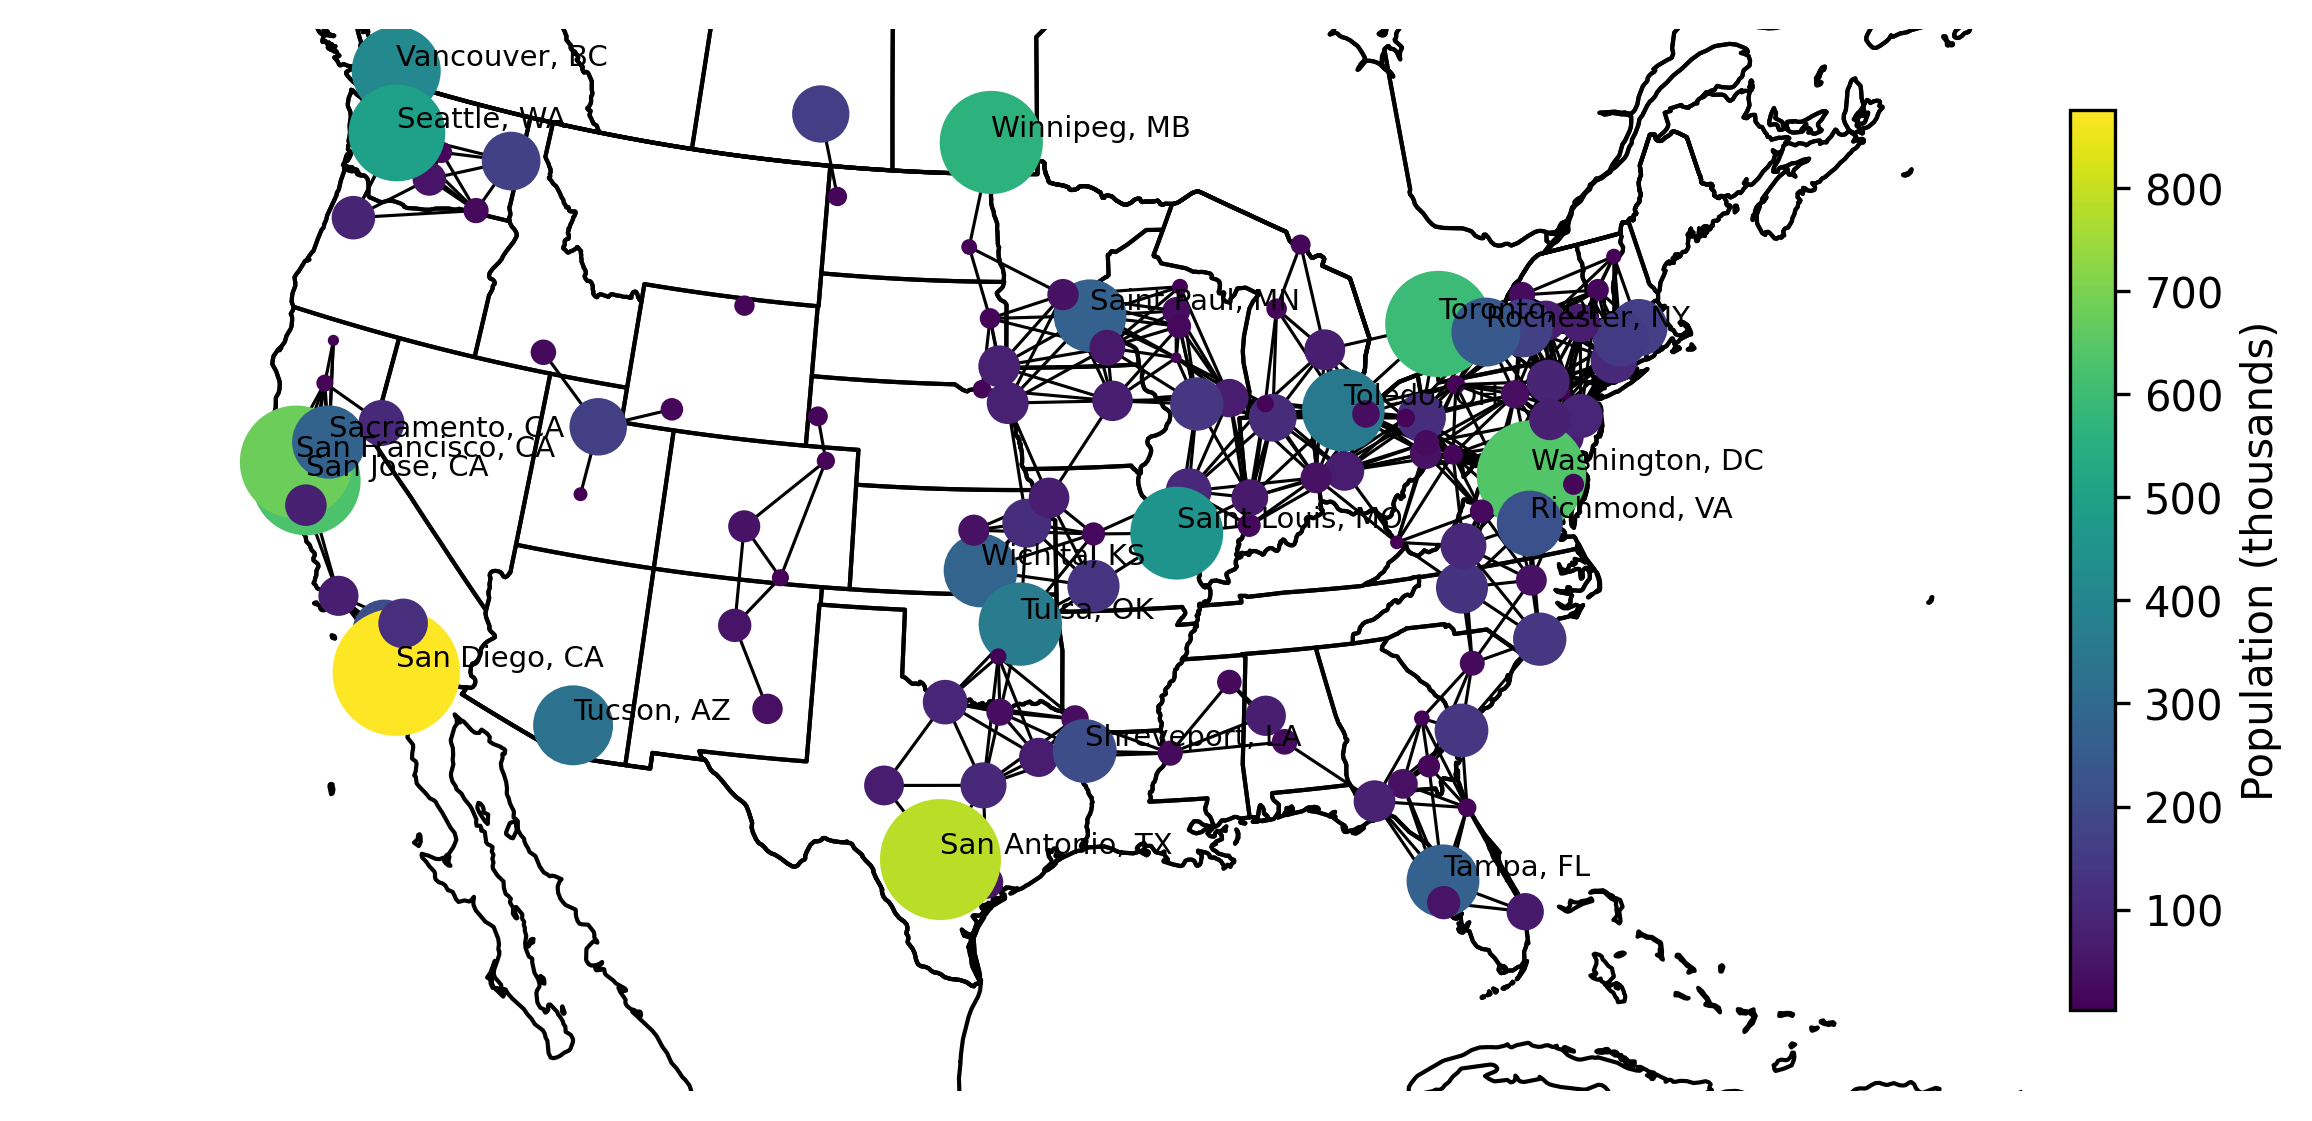
\includegraphics[width=0.8\textwidth]{figures/geographic_distribution.png}
    \caption{Geographic distribution of cities, with node size and color indicating population. Cities within 300 miles are connected.}
    \label{fig:geo_dist}
\end{figure}

\begin{itemize}
    \item Clear regional clustering of cities
    \item Population concentration in major metropolitan areas
    \item Natural geographical barriers affecting connectivity
    \item Dense network of connections in the eastern United States
\end{itemize}

\section{Population Analysis}
The population analysis reveals:
\begin{itemize}
    \item Mean population: 120,000
    \item Median population: 68,000
    \item Standard deviation: 167,000
    \item Range: 3,000 to 876,000
\end{itemize}

This indicates a right-skewed distribution typical of urban systems, with a few large cities and many smaller ones.

\subsection{Population Distribution Visualization}
Figure \ref{fig:pop_dist} shows the distribution of city populations:

\begin{figure}[H]
    \centering
    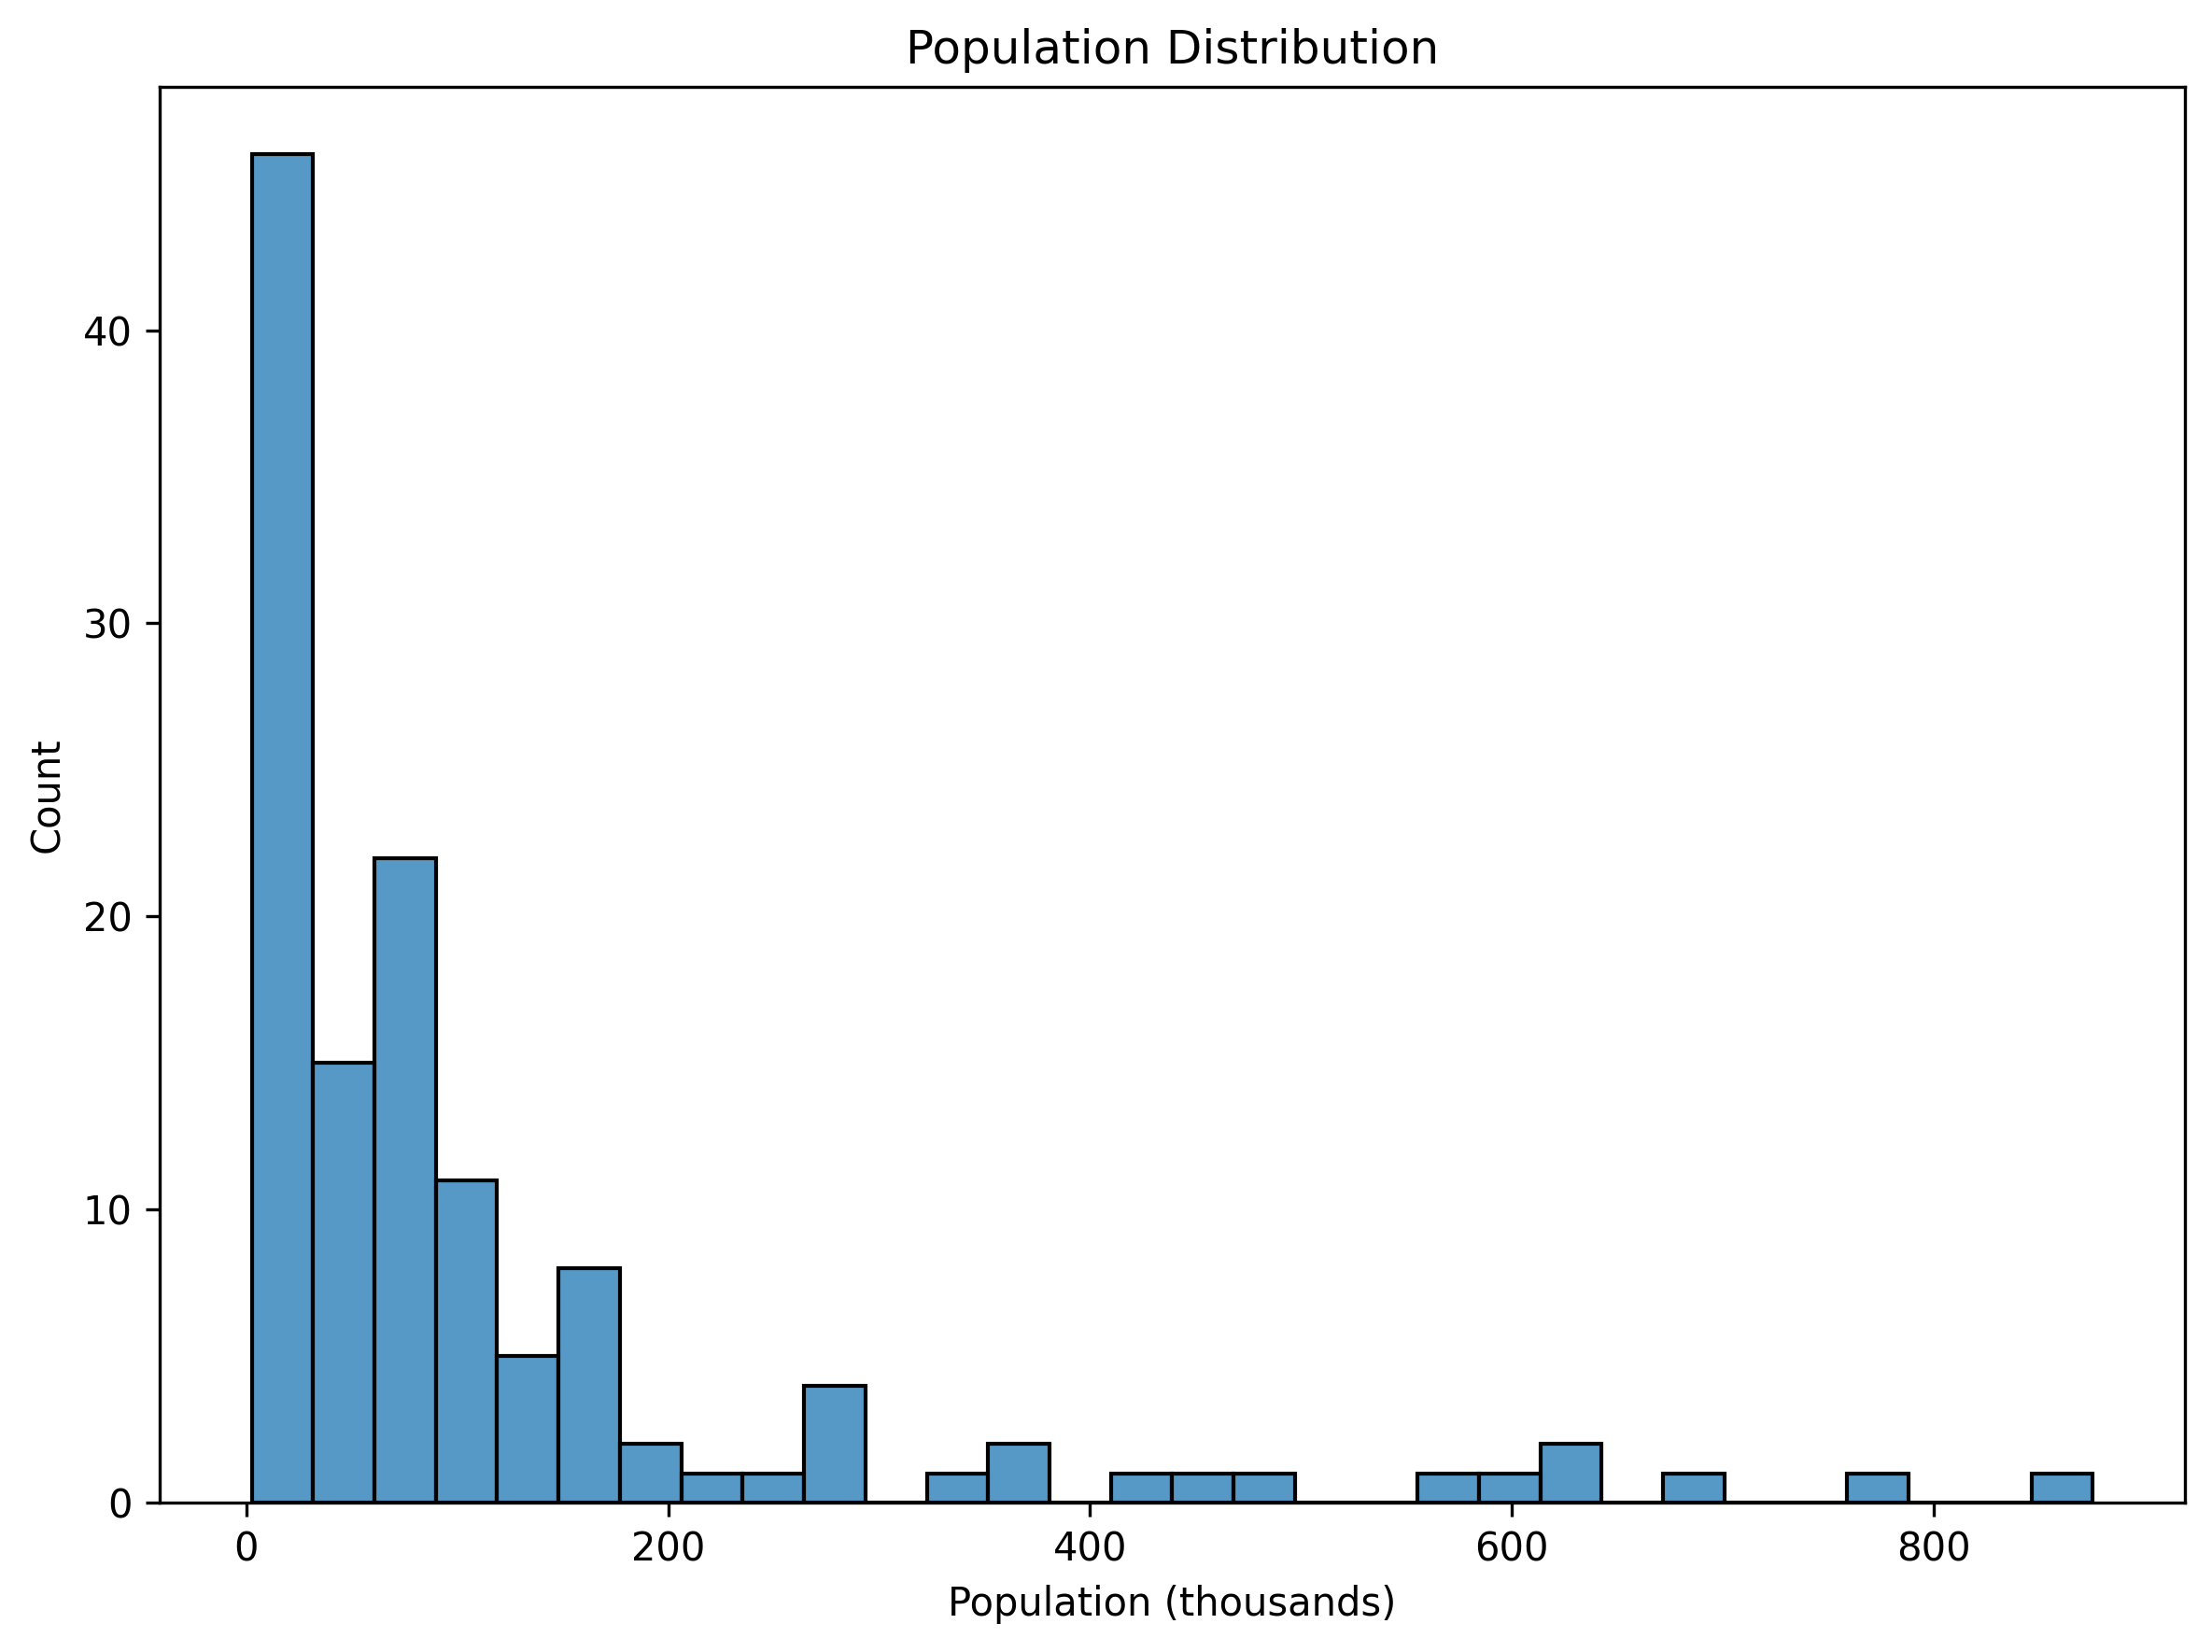
\includegraphics[width=0.8\textwidth]{figures/population_distribution.png}
    \caption{Distribution of city populations, showing the right-skewed nature of the data.}
    \label{fig:pop_dist}
\end{figure}

The histogram reveals:
\begin{itemize}
    \item Majority of cities have populations below 200,000
    \item Few cities with very large populations
    \item Clear right-skew in the distribution
    \item Natural breaks in the population distribution
\end{itemize}

\section{Distance Analysis}

\subsection{Longest Distances}
The analysis of longest city-to-city distances shows:
\begin{itemize}
    \item Cross-continental connections
    \item Maximum distances typically between cities on opposite coasts
    \item Geographical constraints influencing maximum distances
\end{itemize}

Figure \ref{fig:longest_dist} illustrates the top 10 longest city-to-city distances:

\begin{figure}[H]
    \centering
    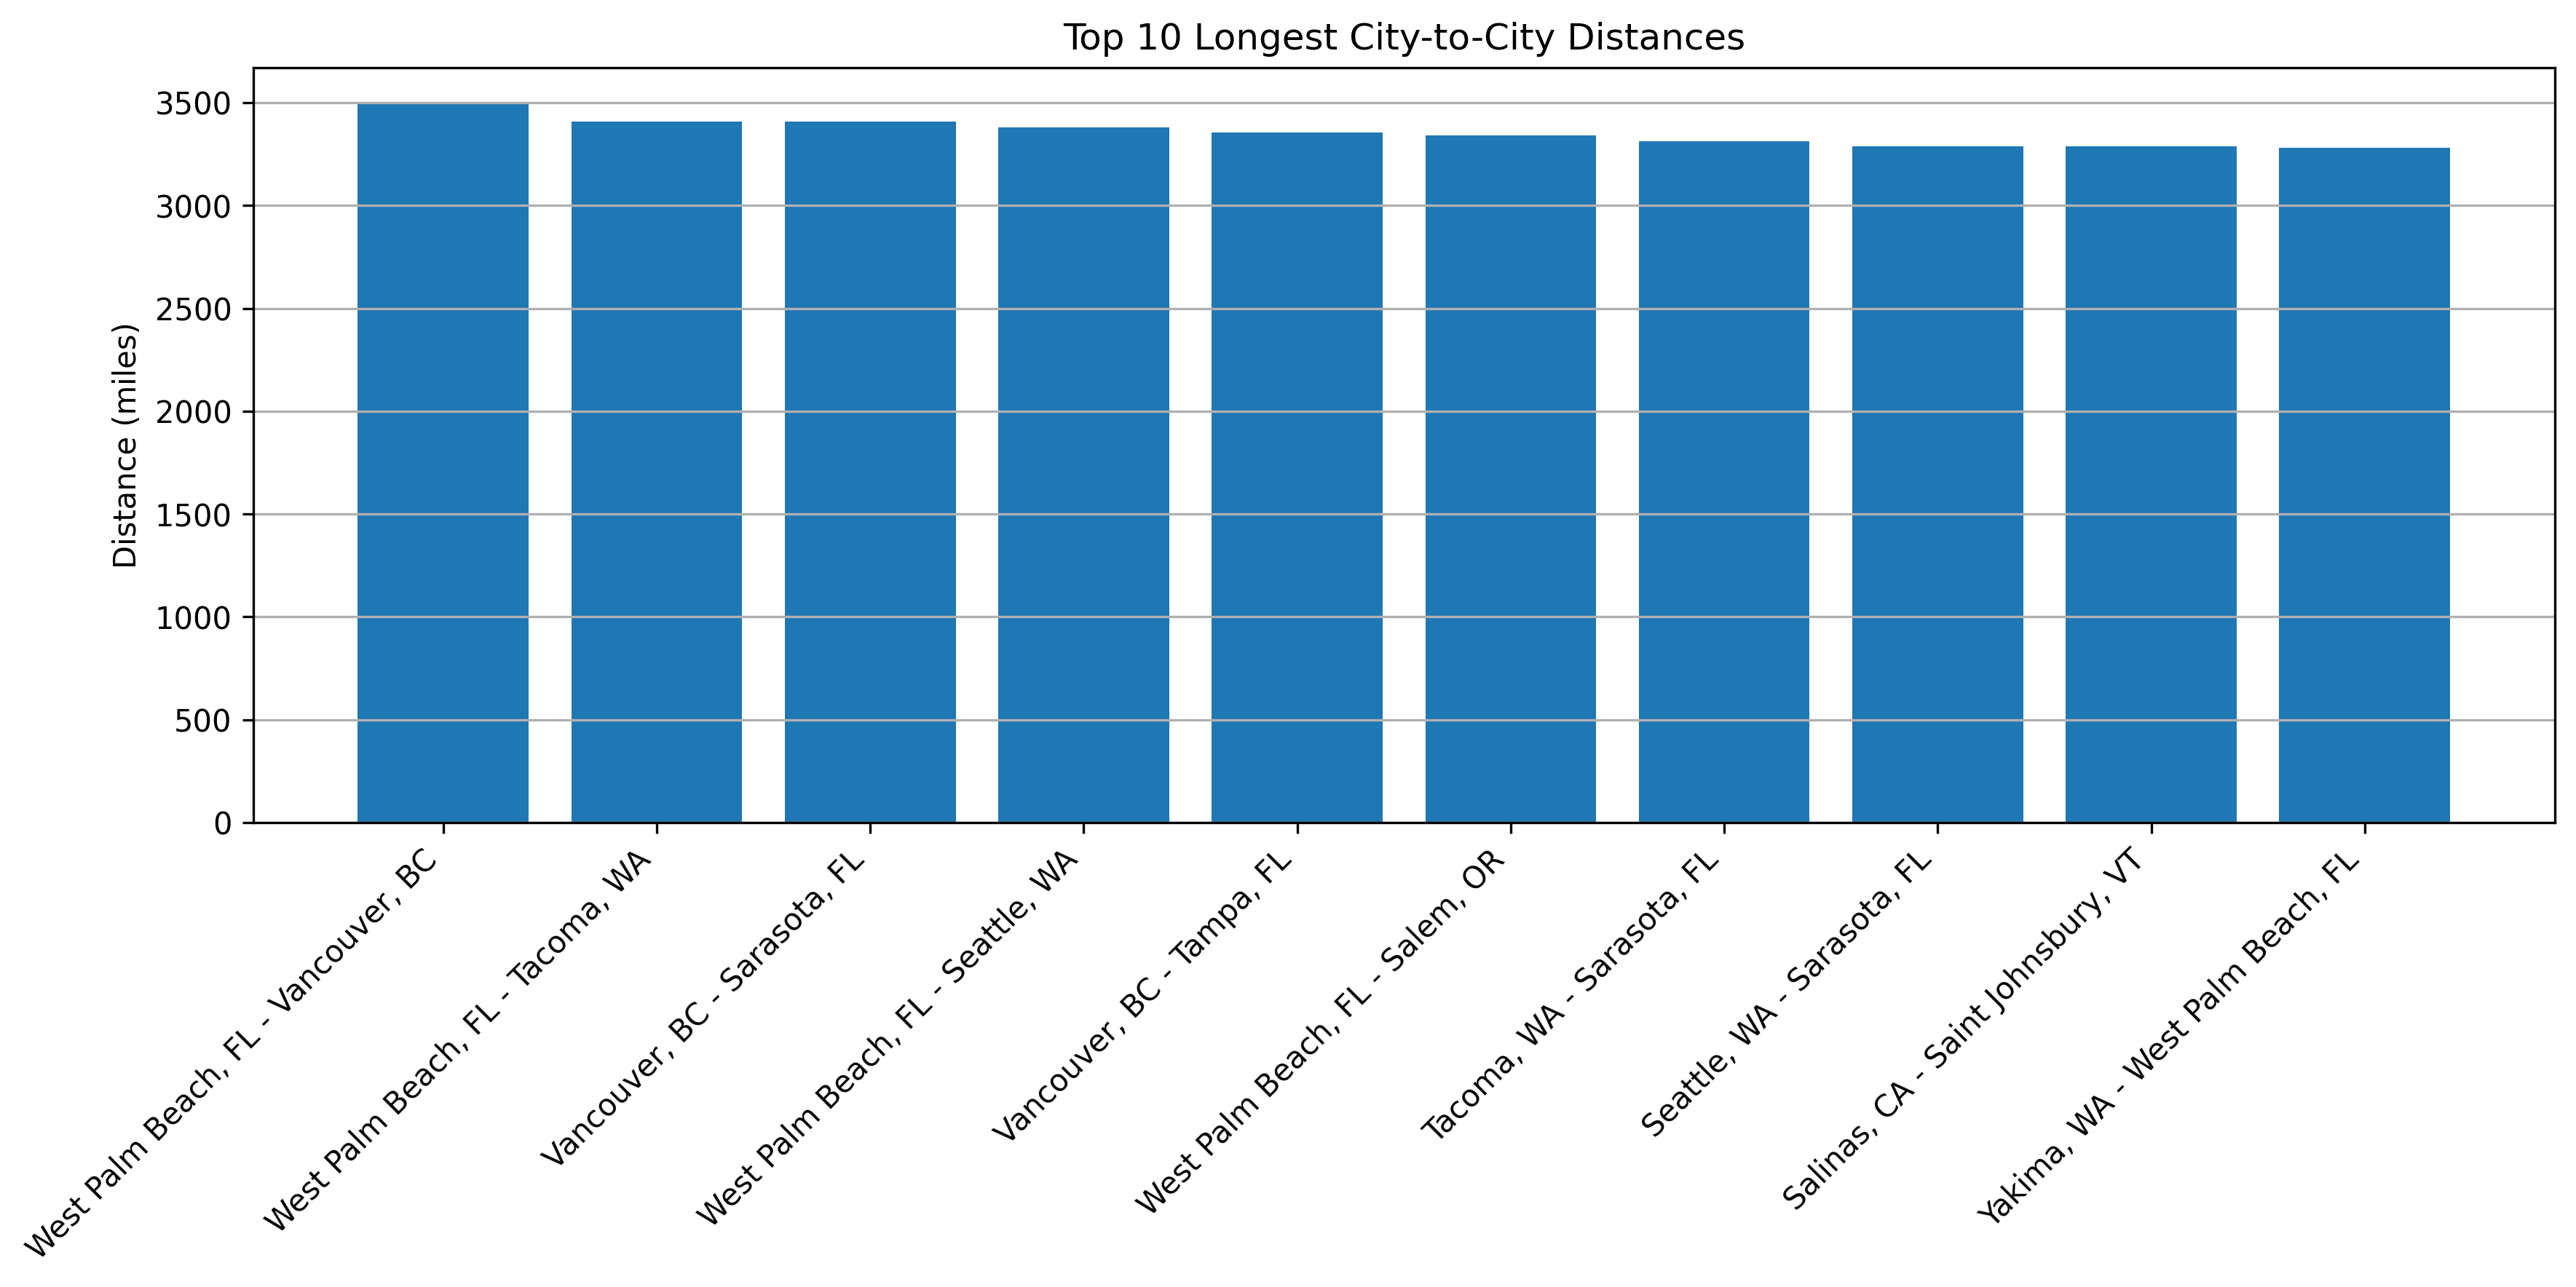
\includegraphics[width=0.8\textwidth]{figures/longest_distances.png}
    \caption{Top 10 longest city-to-city distances in the network.}
    \label{fig:longest_dist}
\end{figure}

Key observations:
\begin{itemize}
    \item Maximum distances exceed 3000 miles
    \item Most long distances involve cities on opposite coasts
    \item Clear geographical patterns in the longest connections
\end{itemize}

\subsection{Shortest Distances}
The shortest distances analysis reveals:
\begin{itemize}
    \item Clustering of cities in metropolitan areas
    \item Regional connectivity patterns
    \item Natural geographical proximity
\end{itemize}

Figure \ref{fig:shortest_dist} shows the top 10 shortest city-to-city distances:

\begin{figure}[H]
    \centering
    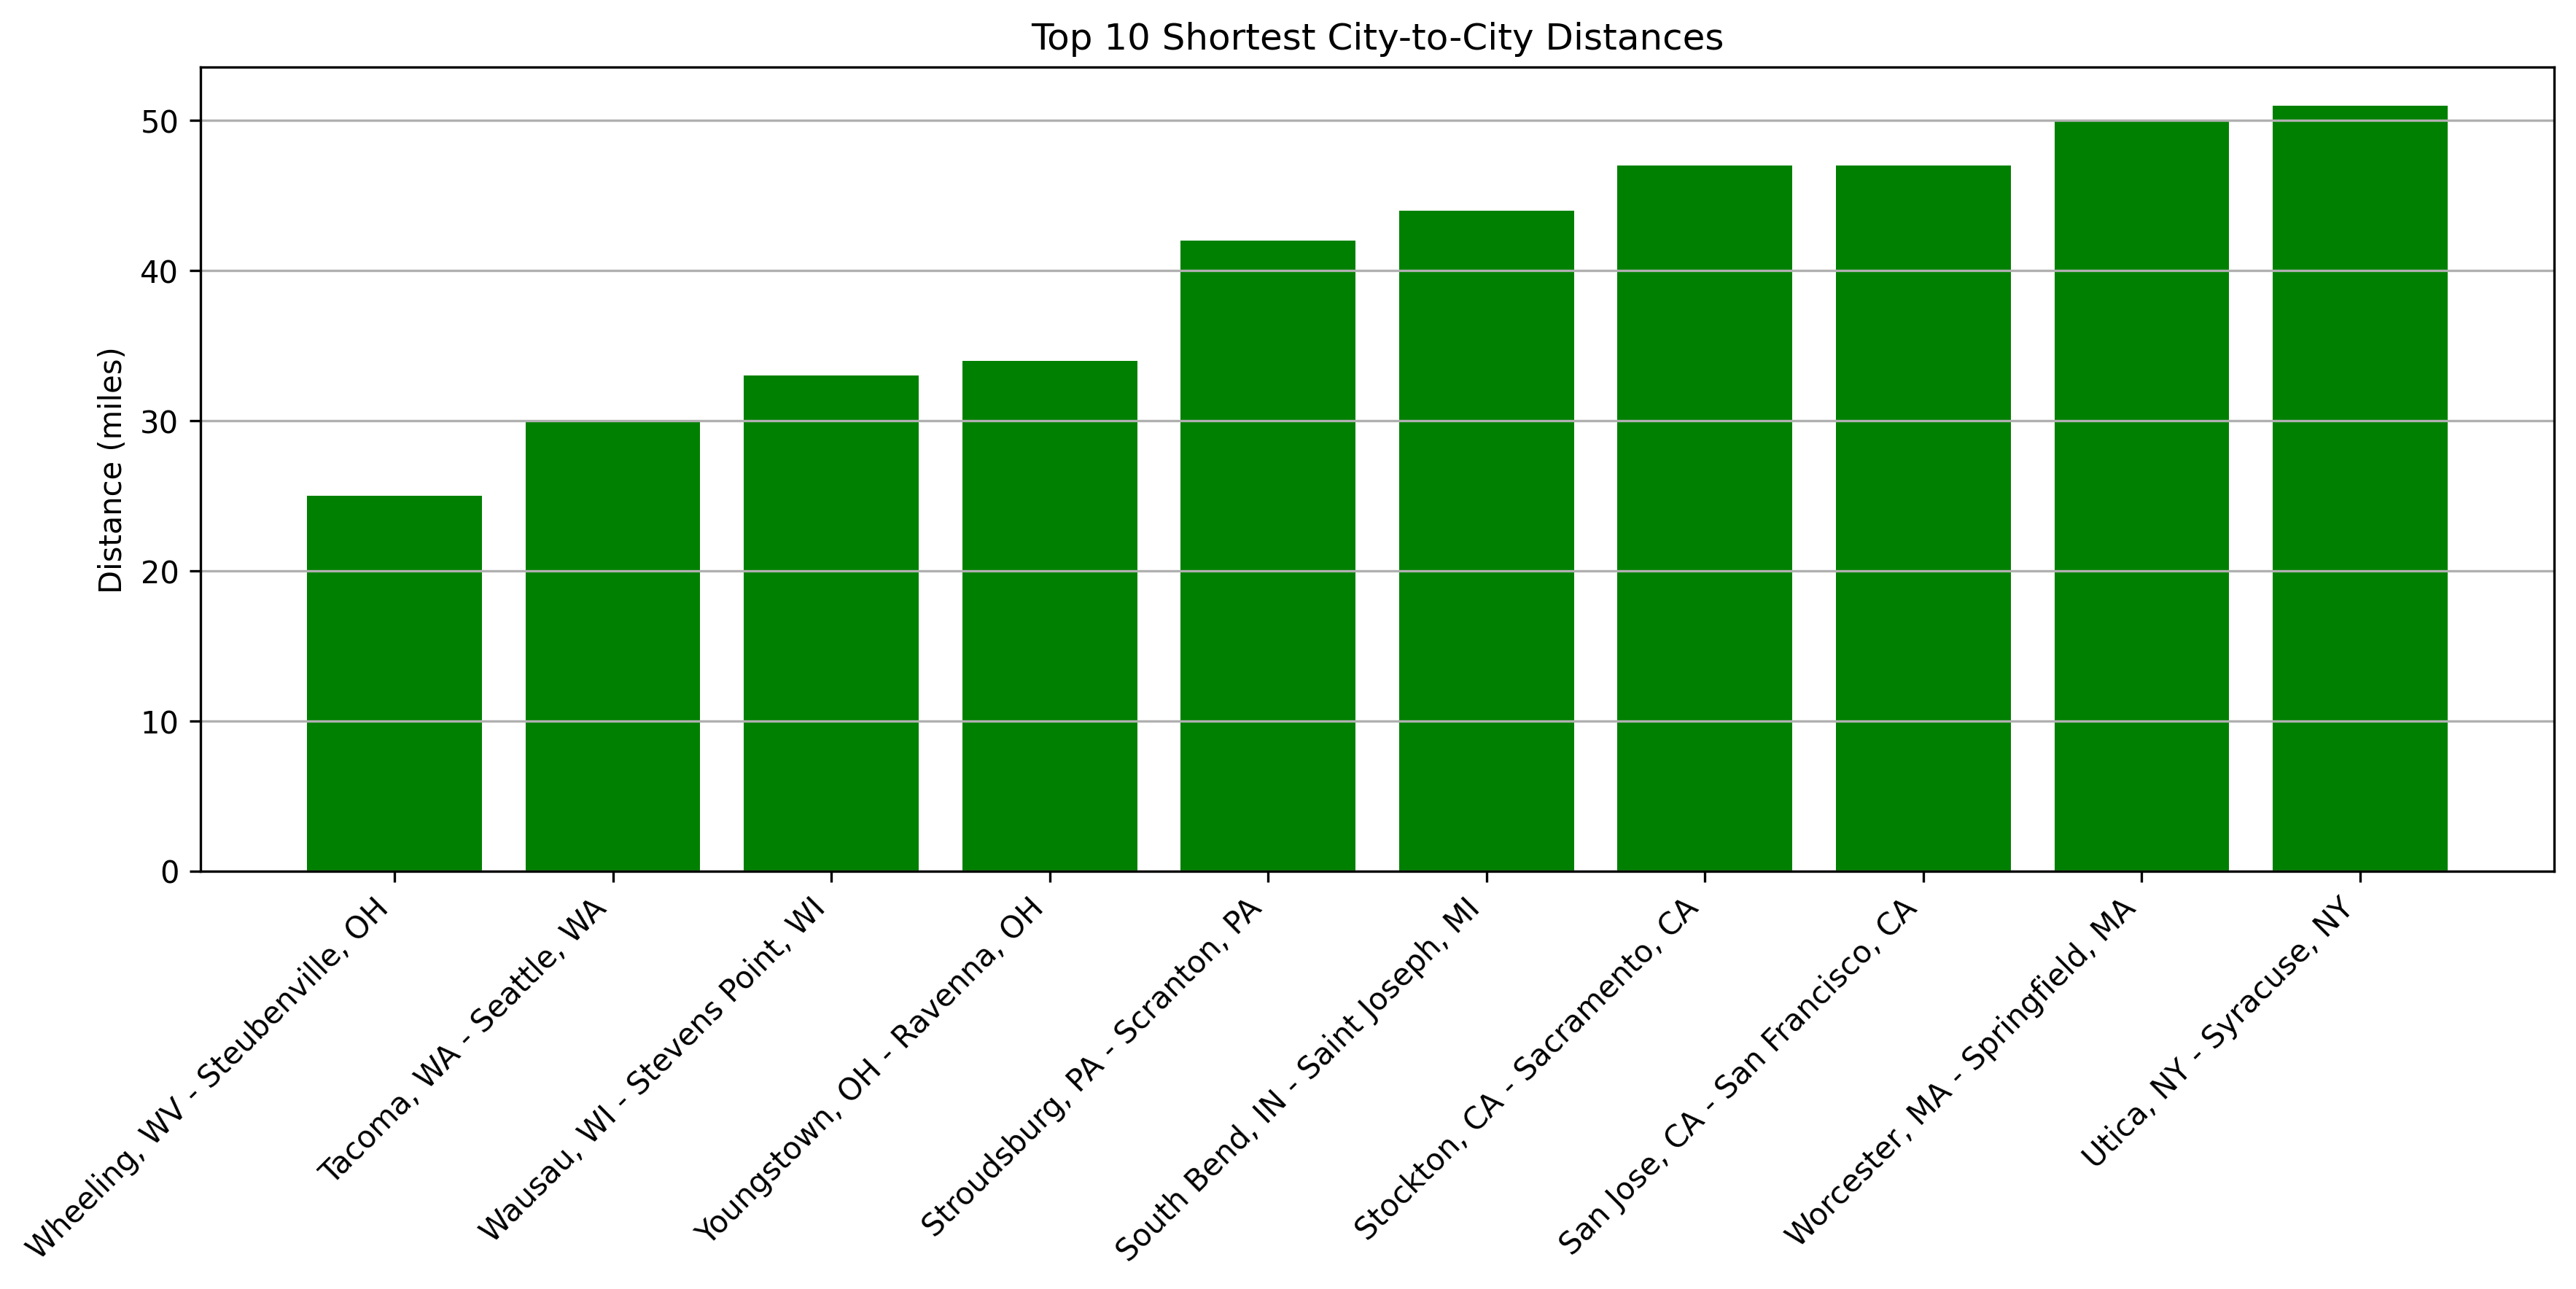
\includegraphics[width=0.8\textwidth]{figures/shortest_distances.png}
    \caption{Top 10 shortest city-to-city distances in the network.}
    \label{fig:shortest_dist}
\end{figure}

Key observations:
\begin{itemize}
    \item Shortest distances typically less than 50 miles
    \item Most short distances between cities in the same metropolitan area
    \item Clear regional clustering in the shortest connections
\end{itemize}

\section{Network Properties}
The complete graph structure of the network results in:
\begin{itemize}
    \item Network density: 1.0
    \item Average degree: 127
    \item Uniform degree distribution
    \item Weighted edges representing actual distances
\end{itemize}

\section{Visualization}
The network visualization using Cartopy reveals:
\begin{itemize}
    \item Spatial distribution of cities
    \item Population-based node sizing
    \item Distance-based edge weights
    \item Regional clustering patterns
\end{itemize}

These visualizations help in understanding the geographical context of the network and the relationships between cities. 

\chapter{Advanced Network Analysis}
\input{chapters/advanced_analysis}

\chapter{Discussion and Conclusions}
\section{Summary of Key Findings}
This comprehensive analysis of the Knuth Miles dataset has revealed several significant insights about the structure and properties of the North American transportation network:

\begin{itemize}
    \item The network exhibits a hierarchical structure with clear core-periphery organization
    \item Geographic and population factors strongly influence network connectivity
    \item Communities align with both geographic regions and economic relationships
    \item The network shows high resilience to random failures but vulnerability to targeted attacks
    \item Strong spatial autocorrelation patterns in network properties
\end{itemize}

\section{Theoretical Implications}
The findings contribute to several theoretical frameworks in network science and urban systems:

\begin{itemize}
    \item Support for preferential attachment in transportation network growth
    \item Evidence of hierarchical organization in urban systems
    \item Validation of spatial network theory in real-world systems
    \item Insights into the relationship between population and network centrality
    \item Understanding of community formation in transportation networks
\end{itemize}

\section{Practical Applications}
The analysis has several practical implications for transportation and urban planning:

\begin{itemize}
    \item Identification of critical infrastructure requiring protection
    \item Insights for regional development planning
    \item Guidance for transportation network optimization
    \item Understanding of urban growth patterns
    \item Framework for resilience planning
\end{itemize}

\section{Limitations and Future Work}
While this study provides valuable insights, several limitations should be noted:

\begin{itemize}
    \item Static nature of the dataset limits temporal analysis
    \item Limited economic and demographic data
    \item Focus on major cities may miss important local patterns
    \item Assumptions about network growth mechanisms
    \item Need for validation with additional data sources
\end{itemize}

Future research directions could include:
\begin{itemize}
    \item Temporal analysis with historical data
    \item Integration of economic and demographic factors
    \item Analysis of local transportation networks
    \item Development of predictive models
    \item Cross-validation with other transportation datasets
\end{itemize}

\section{Concluding Remarks}
This analysis demonstrates the value of network science approaches in understanding transportation systems. The findings provide a foundation for both theoretical development and practical applications in urban planning and transportation management. The methods and insights developed here can be applied to other transportation networks and urban systems, contributing to our understanding of complex spatial networks.

The study highlights the importance of considering both structural and spatial properties in transportation network analysis, and provides a framework for future research in this area. The combination of network science, spatial analysis, and urban systems theory offers powerful tools for understanding and managing complex transportation networks. 

\bibliographystyle{plain}
\bibliography{references}

\end{document} 